\chapter{FUNDAMENTAÇÃO TEÓRICA}

Neste capítulo é apresentada uma revisão de assuntos relacionados na literatura, visando embasamento conceitual, para o entendimento deste trabalho.


\section{Documentação do usuário}

Na Engenharia de Software, a especificação de requisitos é responsável por fazer a ligação entre a engenharia de sistema e o projeto de software. O objetivo da análise de requisitos é fazer uma representação das informações e funcionalidades envolvidas no sistema, de maneira que possa ser entendida e implementada corretamente \cite{PRESSMAN}.

Os requisitos do sistema, funcionais e não funcionais, devem ser descritos de uma forma compreensível aos usuários do sistema, evitando descrições de implementação, que serão especificadas em fases posteriores.

Independente de quais formatos de representação ou modelos de especificação tenham sido utilizados, a especificação de critérios de validação é de extrema importância para a revisão dos requisitos.

Dentre os aspectos a serem considerados em uma validação de requisitos, um importante item é a revisão do Manual Preliminar do Usuário. Este documento define previamente um esboço da utilização do sistema, para que possa ser validado pelo usuário.

Segundo \citeonline{SOMMERVILLE} e \citeonline{PRESSMAN}, esses conceitos são parte da engenharia de requisitos. Entretanto percebe-se que o software, em processo de evolução constante visando se adequar à realidade do usuário, tende-se a distanciar deste tipo de documentação.

Este é um dos problemas que este trabalho tenta resolver, através da utilização de técnicas de teste para manter o sincronismo entre o software e documentação.

\section{Origem dos testes na indústria}

Desde do início da indústria percebeu-se que os produtos precisam estar adequados a especificação. Produtos que são terminados com inconformidades tornam a produção mais lenta, gerando desperdícios como adaptação, retrabalho e refugo. O mesmo ocorre no processo de desenvolvimento de software, onde cada requisito deve atender as especificações solicitadas pelo cliente, caso contrário poderá ter funcionalidades inadequadas ou desnecessárias, que levam aos mesmos problemas da indústria.

A solução utilizada no secúlo XX, foi a inspeção ao final da produção. A indústria ocidental evoluiu ao fazer inspeções proativas (no estoque) e estatísticas por período de tempo. Entretanto o tempo entre a geração do erro e sua identificação diminui a capacidade de identificação da causa raíz dos problemas e de sua solução \cite{CARVALHO}.

Segundo \citeonline{HOLWEG}, em 1918 Sakichi Toyoda implantou em sua indústria de tecelagem uma máquina que verifica a linha de produção. Ao detectar anormalidades, como por exemplo a falta ou quebra da linha, a produção era parada e os operadores avisados, evitando assim a necessidade de operários para monitoramento da produção, e que o produto não atendesse a especificação. Desta maneira o tempo de identifição do problema é curto, evita vários problemas no processo de produção e aumenta as chances de análise e identificação das causas dos problemas.

Entretanto, todo o conhecimento gerado na industria oriental passou desapercebido, sem publicações científicas, até a década de 90, quando se iniciaram pesquisas a este respeito. Sendo assim, até os dias de hoje, percebe-se grandes falhas em empreendimentos nas diversas formas de indústria, inclusive na indústria de software.

\section{Prejuízos na indústria de software}

Software são desenvolvidos a mais de cinquenta anos e ainda tem grandes problemas com a qualidade e garantia de entrega. Segundo \citeonline{CHARETTE}, bilhões de dólares são gastos em projetos  que não são terminados, e 5\% a 15\% dos projetos iniciados serão abandonados antes de serem entregues ou considerados totalmente inadequados logo depois de seu término.

Desenvolver sistemas é caro, e o processo frequentemente sofre dificuldades com as metodologias adotadas, muitas delas não se adequam as atuais exigências do mercado. Por exemplo, o gerente do projeto e os desenvolvedores, devem estar sempre preparados para avaliar as demandas passadas pelos seus clientes (stakeholders) durante o processo de desenvolvimento do sistema. Na etapa de codificação, surgem constantes solicitações de modificações dos requisitos, os quais podem afetar o custo e a qualidade do software \cite{CERPA}.

O maior problema no processo de desenvolvimento é a existência de falhas no sistema, principalmente as detectáveis e previsíveis. Porém, muitas organizações ainda não consideram que a prevenção e detecção de falhas através de testes seja importante, mesmo que possam correr o risco de causar prejuízos ao cliente \cite{CHARETTE}. A tabela \ref{falhas_em_projetos} exemplifica tipos de falha em projetos de desenvolvimento de software é apresentada abaixo.

\begin{table}[ht]
	\centering
	\fontsize{8}{0}
	\caption{Percentual de projetos falhos por fator de falha \cite{CERPA}}
	\label{falhas_em_projetos}
\begin{tabular}{lccc}

\hline

\textbf{Fatores de falha em projetos de software} & \multicolumn{3}{c}{\textbf{Porcentagem de projetos (\%)}}\tabularnewline

\cline{2-4}

& \textbf{In-House} & \textbf{Outsourced} & \textbf{Geral}\tabularnewline

\hline

Data de entrega influenciou no processo & 93,9 & 90,5 & 92,9\tabularnewline

\hline

Projeto estimado por baixo & 83,7 & 76,2 & 81,4\tabularnewline

\hline

Riscos não fora reavaliados, controlados ou gerenciados & 73,4 & 80,9 & 75,7\tabularnewline

\hline

A gerência não foi recompensada por longas horas de trabalho & 81,6 & 57,1 & 74,3\tabularnewline

\hline

Tomada de decisão foi feita sem informações necessárias & 83,7 & 47,6 & 72,9\tabularnewline

\hline

A gerência teve experiência desconfortável & 83,7 & 47,6 & 72,9\tabularnewline

\hline

Clientes não envolvidos na preparação do cronograma & 69,4 & 76,2 & 71,4\tabularnewline

\hline

Risco não está incorporado no planejamento do projeto & 65,3 & 80,9 & 70,0\tabularnewline

\hline

Controle de mudanças não monitorado/negociado efetivamente & 63,3 & 85,7 & 70,0\tabularnewline

\hline

Clientes e usuários tiveram espectativas não realísticas & 69,4 & 66,7 & 68,6\tabularnewline

\hline

Processo não teve revisões ao final de cada fase & 75,5 & 47,6 & 67,1\tabularnewline

\hline

Metodologia não apropriada para o projeto & 71,4 & 52,4 & 65,7\tabularnewline

\hline

Cronograma agressivo afetou a motivação da equipe & 69,4 & 57,1 & 65,7\tabularnewline

\hline

Mudanças no escopo durante o projeto & 67,3 & 57,1 & 64,3\tabularnewline

\hline

Cronograma teve efeito negativo na vida dos elementos da equipe & 71,4 & 42,9 & 62,9\tabularnewline

\hline

Projeto com equipe inadequada para cumprir o cronograma & 63,3 & 57,1 & 61,4\tabularnewline

\hline

Equipe adicionada tardiamente para cumprir um cronograma & 61,2 & 61,9 & 61,4\tabularnewline

\hline

Clientes não dão tempo suficiente para levantar requisitos & 61,2 & 57,1 & 60,0\tabularnewline

\hline

\end{tabular}
\end{table}


\section{Filosofia de Teste de Software}

Teste de software é uma das mais importantes atividades na garantia de qualidade. Segundo \citeonline{PRESSMAN}, a atividade de teste em um projeto de software pode consumir 40\% do esforço total do mesmo e chegar a custar de três a cinco vezes mais que todas as outras etapas da engenharia de software somadas.

A definição comumente aceita da atividade de teste de software é a de que "teste de software consiste de uma série de procedimentos pré-definidos para garantir que o código faça o que ele foi projetado para fazer e não tenha nenhum comportamento não desejado". Porém, \citeonline{MYERS}, aponta para o fato de que o objetivo primário de um teste de software é encontrar erros no código e não provar que o programa atinge aos objetivos: "Teste de software é o processo de se executar um programa com o propósito de descobrir erros".

Muitos programadores assumem uma definição menos eficiente sobre a atividade de teste:

\begin{itemize}
\item A atividade de teste é o processo de demonstrar a inexistência de erros no software
\end{itemize}

Esse pensamento comum é inapropriado pois apesar da atividade de teste poder descobrir defeitos no software, ela é incapaz de mostrar a inexistência destes. No mundo real, é impraticável criar casos de teste para todas as combinações e cenários possíveis para aplicações mais complexas.

\begin{itemize}
\item O propósito da atividade de teste é mostrar que um programa executa suas funções corretamente.
\end{itemize}

Esta definição pode ser considerada incompleta pois mesmo que um programa atinja os objetivos para o qual foi projetado, ainda pode conter erros caso apresente funcionalidades adicionais.

\begin{itemize}
\item Teste de software é o processo de garantir que um programa faz o que foi projetado para fazer.
\end{itemize}

Apesar de uma atividade de teste bem executada poder demonstrar a conformidade entre os requisitos do cliente e as funcionalidades implementadas no software, este é um benefício secundário. Como qualquer outra atividade no processo de desenvolvimento, testes também devem agregar valor ao software, e portanto é importante encontrar defeitos. Neste sentido, a qualidade da atividade de teste será diretamente proporcial ao esforço em encontrar defeitos.

Por tudo isso, percebe-se que os testes de software cumprem uma função ética no processo de desenvolvimento, evitando prejuízos para as organizações ou pessoas. Um exemplo claro disso, é a responsabilidade atribuída ao desenvolvedor do algoritmo presente em um marca-passo, onde qualquer falha pode causar graves prejuízos ao usuário.

Portanto, para conduzir os testes efetivamente, existe toda uma complexidade advinda da variedade de algorítmos que precisarão ser testados. Várias técnicas propostas para endereçar os testes de algorítmos são apresentadas nos tópico a seguir.


\section{Testes de software}

O desenvolvimento de sistemas de software deve ser acompanhado de testes que contemplem tanto o funcionamento interno dos componentes como o comportamento esperado das funcionalidades. Estas atividades são conhecidas como testes de caixa branca e caixa preta, respectivamente. \citeonline{PRESSMAN} conceitua estes paradigmas de teste conforme abaixo:

\subsection{Testes caixa branca}

Este método de teste verifica internamente o funcionamento das estrutura de dados do sistema, testando os caminhos possíveis e as decisões lógicas existentes. O procedimento de se testar internamente é útil para detectar erros lógicos em funções secundárias, que usualmente não levam a mesma atenção que as principais, além de mostrar caminhos não imaginados no fluxo de execução e erros tipográficos.

\subsection{Testes de caixa preta}

Os testes do tipo caixa preta são responsáveis por testar os requisitos funcionais, desconsiderando o funcionamento interno do componente de software. Nos testes de caixa preta, o desenvolvedor cria um conjunto de entradas de dados e verifica a saída esperada. Deste maneira, procura-se detectar erros na implementação dos requisitos, como na interface de usuário, inicialização e término do sistema, desempenho e estruturas de dados.

\subsection{Testes de regressão}
Indepenndete da estrategia de testes, sempre que alteracoes forem realizadas no codigo fonte, efeitos colaterais podem ser criados em outras partes do codigo. Portanto, ainda corroborando com o raciocínio de \opcit{PRESSMAN}, o software precisa ser totalmente testado após cada alteração produzida. Testes de regressão buscam levar o software às falhas que revelem onde esses defeitos foram provocados.

\subsection{Tipos de testes}

O alvo a ser testado também requer que o programador aplique uma política de testes específica. Por exemplo ao testar métodos, classes, módulos, sistemas, a abordagem deve variar conforme o grau de abstração, a complexidade e o risco inerente.

\begin{itemize}
\item \textbf{Testes de unidade:} Estes testes são baseados na caixa branca e testam a menor unidade do software possível, como um módulo ou um objeto, visando detectar erros na implementação interna do mesmo. Um teste de unidade deve testar apenas um componente isoladamente, buscado portanto a coesão necessária para garantir sua funcionamento.
\end{itemize}

\begin{itemize}
\item \textbf{Testes de integração:} Somente os testes de unidade não são suficientes para garantir que todos os componentes de um sistema irão funcionar perfeitamente quando integrados. Um componente do sistema pode ter um comportamento inesperado, adverso, sobre outro. Os testes de integração detectam erros nos contratos entre os módulos, definindo a estrutura pré-definida do software.
\end{itemize}

\begin{itemize}
\item \textbf{Teste de validação:} Esta estratégia de teste pode ser definida pela validação dos requisitos do usuário, são os testes finais do software. Estes testes validam os critérios de aceitação que irão informar se os requisitos corretos foram implementados no sistema. Por exemplo, quando um cliente utiliza o sistema e encontra as funcionalidades requeridas.
\end{itemize}

\section{Formato \textit{YAML}}
\label{sec:yaml}

O \textit{YAML} é um formato de serialização de dados que pode ser facilmente entendível por humanos e ao mesmo tempo é flexível e facilmente manipulável. Ele aceita representação para as estruturas de listas, dicionários e valores simples, como texto e inteiros \cite{YAML}.

Além disso, este formato utiliza uma notação baseada em indentação e um conjunto de caracteres para demarcar sua estrutura. Abaixo serão listadas algumas outras características deste formato.

\begin{itemize}
\item A estrutura do documento é composto por indentação com espaços em branco e não é permitido o uso de caracteres de tabulação para a indentação.

\item Os valores simples não levam as aspas, mas podem ser incluídas as aspas duplas ou aspas simples.

\item Os membros das listas são encabeçados por um traço nos títulos e com um membro em cada linha, ou entre colchetes e separados por uma vírgula e espaço.
\end{itemize}

O Código \ref{lst:codigo21} exemplifica as caracteristicas descritas anteriormente.

{\singlespace
\begin{lstlisting}[caption=Estrutura do código \textit{YAML},language=bash,label={lst:codigo21}]
titulo: "Exemplo de listas"
data: Julho de 2012

listagem_1: [Tiago, Natanael]

listagem_2:
  - Tiago
  - Natanael
\end{lstlisting}
}

\section{\textit{Psych}}

\textit{Psych} \cite{PSYCH} é uma biblioteca open-source e multiplataforma, implementada em \textit{Ruby}, para a análise e geração de YAML.

Esta biblioteca é de uso bastante simples, como pode ser visto no exemplo abaixo (Código \ref{lst:codigo_psych}), em que uma string em formato YAML é analisada e transforma em uma estrutura de dados em Ruby, com listas, dicionários e valores simples:

{\singlespace
\begin{lstlisting}[caption=Biblioteca \textit{Psych}, language=Ruby,label={lst:codigo_psych}]
yaml = <<-YAML
livros:
  Tecnicos: [Programming Ruby 1.9]
  Literatura: [O Festim dos Corvos, Morte dos Reis]
YAML

puts Psych.load(yaml)
# => {"livros" => {
#      "Tecnicos" => ["Programming Ruby 1.9"],
#      "Literatura" => ["O Festim dos Corvos", "Morte dos Reis"]}}
\end{lstlisting}
}

\section{\textit{Hashr}}

\textit{Hashr} \cite{HASHR} é uma pequena e simples biblioteca em \textit{Ruby}, que extende a classe nativa \textit{Hash} da linguagem, adicionando algumas características que tornam o uso da estrutura de dicionários mais fácil, elegante e menos propensa a erros.

Em um objeto da classe Hashr, diferentemente da classe nativa Hash, os valores do dicionário podem ser acessados de forma direta, bastando apenas chamar o método de mesmo nome do índice que o valor correspondente é retornado (Código \ref{lst:codigo_hashr}).

Da mesma forma, esta biblioteca também permite a atribuição dos valores, bem como a criação de novos pares no dicionário. Além de aceitar também, métodos com os nomes dos índices acrescentados do caractere "?", que retorna sempre um valor booleano, \textit{true} se o índice existir e \textit{false} caso contrário.

Uma característica bastante útil nesta biblioteca é que os dicionários aninhados são automaticamente instanciados pela mesma classe Hashr. Isto é, ao adicionar novos dicionários dentro de um objeto Hashr usando a sintaxe nativa da linguagem, eles também serão objetos Hashr, permitindo o mesmo estilo na manipulação dos mesmos.

{\singlespace
\begin{lstlisting}[caption=Exemplo do uso da classe \textit{Hashr} retirado da página do projeto, language=Ruby,label={lst:codigo_hashr}]
config = Hashr.new('foo' => { 'bar' => 'bar' })

config.foo?     # => true
config.foo      # => { :bar => 'bar' }

config.foo.bar? # => true
config.foo.bar  # => 'bar'

config.foo.bar = 'bar!'
config.foo.bar # => 'bar!'

config.foo.baz = 'baz'
config.foo.baz # => 'baz'\end{lstlisting}
}


\section{JavaScript}

JavaScript (JS) surgiu em 1995, com o objetivo de validar a entrada de dados em páginas web, pois neste período nem todos os dados eram tratados pelo servidor. A capacidade de lidar com algumas validações básicas no cliente, era uma característica nova e excitante, num momento em que o uso de modems de telefone estava crescendo, e a lenta velocidade das conexões tornavam o acesso a web um exercício de paciência \cite{ZAKAS}.

Segundo \citeonline{PIRES}, JS é uma linguagem de programação, pequena, leve, orientada a objetos e multi-plataforma (Código \ref{lst:codigo22}). Mais conhecida como uma linguagem de script para páginas web, mas também muito bem utilizada em dispositivos móveis modernos, como celulares e tablets. Hoje em dia, JS é uma linguagem que pode ser utilizada em qualquer aspecto, desde aplicações no lado cliente (aplicações de front-end), como do lado servidor (aplicações server-side).

{\singlespace
\begin{lstlisting}[caption=Classe Pessoa em \textit{JavaScript},language=Java,label={lst:codigo22}]
<script language="javascript">
function Pessoa () {
    var nome;
    var sobrenome;

    this.getNome = getNome;
    this.getSobrenome = getSobrenome;
    this.setNome = setNome;
    this.setSobrenome = setSobrenome;
    this.nomeCompleto = nomeCompleto;

    function getNome () {
        return nome;
    }

    function getSobrenome () {
        return sobrenome;
    }

    function setNome (_nome) {
        nome = _nome;
    }

    function setSobrenome (_sobrenome) {
        sobrenome = _sobrenome;
    }

    function nomeCompleto () {
        return getNome() + " " + getSobrenome();
    }
}
</script>
\end{lstlisting}
}

Portanto, esta linguagem pode interagir com todo conteúdo da página e a janela do navegador, sem realizar requisições ao servidor da aplicação, desta forma oferece uma dinâmica maior às páginas, maior velocidade ao usuário e maior flexibilidade ao programador.

\section{\textit{jQuery}}
\label{sec:jquery}

Nos dias de hoje a \textit{internet} é um ambiente dinâmico, e os seus usuários exigem cada vez mais interatividade e estilo. Para construir interessantes sites interativos, os desenvolvedores voltam-se para o uso bibliotecas \textit{JavaScript} como \textit{jQuery}. Esta biblioteca permite automatizar tarefas comuns e simplificar as complicadas. Uma das razões para a popularidade do \textit{jQuery} é sua capacidade de ajudar em uma ampla gama de tarefas.

Segundo \citeonline{CHAFFER} muitos dos conceitos da biblioteca são baseados na estrutura do código \textit{HTML} e \textit{Cascading Style Sheets} (CSS). Suas principais características podem nos ajudar a realizar as seguintes tarefas:

\begin{itemize}
\item Acessar os elementos da página: Sem utilizar uma biblioteca \textit{JavaScript} que facilite a seleção de elementos da página, desenvolvedores precisam escrever complexos scripts utilizando a estrutura do \textit{Document Object Model} (DOM). Através desta biblioteca, é possível utilizar um eficiente mecanismo de seleção dos elementos.

\begin{center}
\textit{\$('div.content').find('p');}
\end{center}

\item Alterar a aparência da página: CSS oferece uma poderosa maneira de alterar a aparência de páginas web. Com \textit{jQuery} os desenvolvedores podem alterar dinamicamente as propriedades do CSS da página, mesmo que ela já tenha sido carregada.

\begin{center}
\textit{\$('ul > li:first').addClass('active');}
\end{center}

\item Manipular o conteúdo da página: \textit{jQuery} pode modificar o conteúdo da página sem maiores problemas. É possível alterar textos, adicionar ou trocar imagens, re-ordenar listas e até adicionar novos elementos na página, tudo isso com uma \textit{Application Programming Interface} (API) fácil de usar \cite{JQUERY-API}.

\begin{center}
\textit{\$('\#container').append('<pre>News</pre>');}
\end{center}

\item Responder a interação do usuário: A biblioteca oferece uma maneira simples de interceptar a vasta gama de eventos que o usuário pode disparar, como por exemplo, o evento de clicar em um \textit{link}.

\begin{center}
\textit{\$('button.show-details').click(function() \{ \$('div.details').show(); \});}
\end{center}

\item Executar requisições assíncronas: Esta técnica é chamada de AJAX, o que significa \textit{Asynchronous JavaScript and XML}, a qual possibilita a comunicação cliente-servidor. Desta maneira o desenvolvedor pode executar chamadas ao servidor sem recarregar a página.

\begin{center}
\textit{\$('div.details').load('more.html \#content');}
\end{center}

\item Solucionar incompatibilidades de navegadores: Esta biblioteca é \textit{cross-browser}, o que significa a total compatibilidade de sua API com os atuais navegadores.
\end{itemize}

Portanto, a utilização desta biblioteca facilita o desenvolvimento de aplicações web e diminui a probabilidade de erros, causados pela divergência de padrões existentes entre os navegadores.

\section{\textit{Amberjack}}
\label{sec:amberjack}

\textit{Amberjack} (AJ) é uma biblioteca de código aberto que você pode usar para criar \textit{tours} - tutoriais guiados - que orientam os visitantes do seu site. A idéia básica é explicar as páginas existentes do seu site através de um texto (como este). O texto explicativo é exibido em uma caixa de diálogo uma camada acima da sua página \textit{web} (Figura \ref{figura_22}). AJ foi criado com ênfase na flexibilidade e na facilidade de customização.

\begin{figure}[ht]
    \centering
    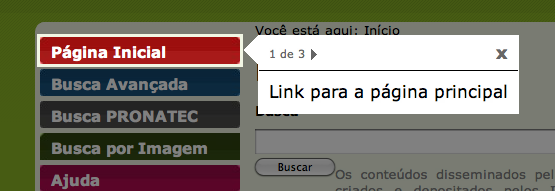
\includegraphics[width=0.9 \textwidth]{figuras/figura_33}
    \caption{\textit{Tour} gerado pela biblioteca \textit{Amberjack}}
    \label{figura_22}
\end{figure}

Para utilizar esta biblioteca não é necessário amplo conhecimento de \textit{JavaScript}, você só precisa adicionar um código \textit{HTML} a sua página web. Este código descreve cada passo que será realizado na página. O código é organizado por um estrutura de "div" aninhados e atributos que descrevem propriedades do cenário (Código \ref{lst:codigo22}).

{\singlespace
\begin{lstlisting}[caption=Estrutura do código \textit{HTML} do \textit{Amberjack},language=HTML,label={lst:codigo23}]
<div class="ajTourDef" id="MeuExemplo" style="display:none" title="http://feedback.exemplo.com/">
  <div title="http://exemplo.com/">
    <div title="id:'elemento1',padding:0,trbl:'ltb'">
      <strong>Primeiro passo</strong>
      <br />Primeiro passo na página inicial
    </div>
    <div title="id:'elemento2',padding:0,trbl:'ltb'">
      Segundo passo
      <br />Próximo passo será em outra página.
    </div>
  </div>
  <div title="http://exemplo.com/noticias">
    <div title="id:'markerColor',padding:0,trbl:'ltb'">
      <strong>Fim do exemplo</strong>
      <br />Página de notícias.
    </div>
  </div>
</div>
\end{lstlisting}
}

A primeira linha define uma ``div'' responsável pelo tutorial. Nesta ``div'' são definidos dois importantes atributos, id e title. O id é o identificador do tutorial, o qual deve ser utilizado para iniciá-lo, já o title define a url que o usuário será redirecionado ao terminar o tutorial.

Nas linhas 2 e 12, são criadas as ``div'' que definem o contexto no qual os passos serão realizados. O atributo title define a url na qual os passos serão executados.

Dentro de cada uma destas ``div'' que estabelecem o contexto de execução, são criadas as estruturas finais. Cada ``div'' que encontra-se dentro de um contexto, tem dois importantes atributos, id e trbl. Eles são reponsáveis por definir qual elemento da página será destacado e qual será a posição da caixa de diálogo \cite{AJ}. O conteúdo de cada uma delas será o texto exibido no \textit{tour}.

Por fim, após definir todos os cenários que deseja inserir um \textit{tour}, o mesmo pode ser iniciado a partir da passagem de um parâmetro na url:

\begin{center}
\textit{http://exemplo.com/?tourId=MeuExemplo\&skinId=Safari}
\end{center}







\section{\textit{Ruby}}

A linguagem de programação \textit{Ruby} \cite{RUBY} foi criada no Japão, e desde então seu uso vem crescendo cada vez mais ao redor do mundo com uma comunidade forte e ativa. O objetivo de Matsumoto, era criar uma linguagem que fosse agradável ao desenvolvedor e que possibilitasse uma maior produtividade com o menor trabalho possível.

\textit{Ruby} é uma linguagem open-source e multiplataforma, o que possibilita, além do seu uso em diversos ambientes diferentes, o surgimento de um grande número de bibliotecas criadas pela comunidade de desenvolvedores e até outras implementações da própria linguagem.

Existem várias versões do Ruby, sendo a oficial conhecida como RMI (\textit{Matz’s Ruby Interpreter}). Outras importantes versões são a \textit{Rubinius} \cite{RUBINIUS} - uma implementação com grande parte escrita usando o próprio \textit{Ruby} -  e a \textit{jRuby} \cite{JRUBY} - uma implementação em Java, executada na própria JVM.

Esta linguagem de script tem tipagem forte e dinâmica, além de ser totalmente orientada a objetos.  A Orientação a objetos no projeto desta linguagem é notável, todos os elementos manipulados no uso desta linguagem são objetos, como os tipos simples e as próprias classes \cite{THOMAS}.

Tipagem forte significa que os tipos de dados são bem definidos, existindo uma distância maior entre o comportamento dos tipos existentes, enquanto que numa linguagem de tipagem fraca, eles estão mais próximos. Uma linguagem popular com tipagem fraca é o \textit{JavaScript}, no exemplo a seguir (Código \ref{lst:codigo_tipagem_fraca}) um tipo \textit{string} é somado a um tipo \textit{number}, e o resultado é uma \textit{string}.

{\singlespace
\begin{lstlisting}[caption=Tipagem fraca no \textit{JavaScript}, language=Java, label={lst:codigo_tipagem_fraca}]
string = "lorem ipsum"
number = 123
string + number // => "lorem ipsum123"
\end{lstlisting}
}

O mesmo código em \textit{Ruby} gera um erro, visto que a definição dos tipos são mais distintas (código \ref{lst:codigo_tipagem_forte}).

{\singlespace
\begin{lstlisting}[caption=Tipagem forte no \textit{Ruby}, language=Java, label={lst:codigo_tipagem_forte}]
string = "lorem ipsum"
number = 123
string + number # => TypeError: can't convert Fixnum into String
\end{lstlisting}
}

Em linguagens de tipagem estática, como o \textit{Java}, o tipo do valor que uma variável pode receber, deve ser previamente declarado (Código \ref{lst:codigo_tipagem_estatica}).

{\singlespace
\begin{lstlisting}[caption=Tipagem estática no \textit{Java}, language=Java, label={lst:codigo_tipagem_estatica}]
  public class Main {
      public static void main(String[] args) {
          int integer = 123;
          String string = "lorem ipsum";
      }
  }
\end{lstlisting}
}

Já em linguagens de tipagem dinâmica, como o \textit{Ruby}, as variáveis são meras referências aos objetos, podendo estes ser de qualquer tipo existente (Código \ref{lst:codigo_tipagem_dinamica}). Linguagens com tipagem dinâmica tendem a ser mais flexíveis, dando mais liberdade ao programador.

{\singlespace
\begin{lstlisting}[caption=Tipagem dinâmica no \textit{Ruby}, language=Ruby, label={lst:codigo_tipagem_dinamica}]
  integer = 123
  string = "lorem ipsum"
  var = 10.50
  var = [1, 2]
  var = {key: "value"}
\end{lstlisting}
}

\textit{Ruby} é expressivo, sua sintaxe simples possibilita um código legível e elegante. Em \textit{Ruby}, todas as classes são abertas, podendo ser extendidas facilmente em tempo de execução. Outro conceito muito presente nesta linguagem é a metaprogramação (código que raciocina sobre código), o que torna esta muito poderosa, facilitando por exemplo a criação de DSL’s expressivas.

A sintaxe direta e descomplicada da linguagem, bem próxima do inglês, torna o ato de programar menos doloroso e mais divertido. Em poucas linhas, pode-se criar uma classe e métodos de atribuição e retorno dos atributos (Código \ref{lst:codigo_legibilidade}).

{\singlespace
\begin{lstlisting}[caption=Exemplo de legibilidade em código \textit{Ruby}, language=Ruby, label={lst:codigo_legibilidade}]
  class Human
    attr_accessor :name, :age

    def initialize(args = {})
      @name = args[:name]
      @age = args[:age]
    end
  end

  Human.new name: 'Arya', age: 9
\end{lstlisting}
}

Em seguida (Código \ref{lst:codigo_metaprogramacao}) pode-se ver um exemplo do uso da metaprogramação. Se um método não existente for executado em uma instância da classe \textit{Car}, ele será criado dinamicamente, com a funcionalidade de retornar e atribuir um atributo com o mesmo nome do método executado.

{\singlespace
\begin{lstlisting}[caption=Metaprogramação em \textit{Ruby}, language=Ruby, label={lst:codigo_metaprogramacao}]
  class Car
    def initialize(&block)
      instance_eval(&block) if block_given?
    end

    def method_missing(method, *args)
      method = method.to_s.chop! if method.to_s.end_with? "="
      instance_eval <<-RUBY
        if args.any?
          @#{method} = args.first
          def #{method}
            @#{method}
          end
        else
          super
        end
      RUBY
    end
  end

  car = Car.new

  car.color = "Black"
  car.color # => Black

  car.whatever = "chunky bacon"
  car.whatever # => chunky bacon
\end{lstlisting}
}

DSL (linguagem específica de domínio) é uma linguagem dedicada a resolver um tipo específico de problema, com um estrutura e sintaxe próprios para o ambiente onde ela se destina a trabalhar. Um exemplo de DSL é a linguagem SQL (Linguagem de Consulta Estruturada), que foi desenvolvida especificamente para a manipulação de bancos de dados relacionais, e não é própria para outros propósitos se não este.

No códido abaixo, (Código \ref{lst:codigo_factory_girl}), pode ser observado a DSL da biblioteca de fábrica de objetos \textit{factory\_girl}, implementada em \textit{Ruby}.

{\singlespace
\begin{lstlisting}[caption=DSL da biblioteca \textit{factory\_girl}, language=Ruby, label={lst:codigo_factory_girl}]
  factory :usuario do
    sequence(:email) { |n| "usuario%s@gmail.com" % n }
    password '12345678'
    nome_completo 'Linus Torvalds'
  end
\end{lstlisting}
}

Outra vantagem no uso desta linguagem é a quantidade disponível de ferramentas desenvolvidas pela comunidade, como frameworks e bibliotecas de teste automatizados.

O uso de testes automatizados é levado muito a sério na comunidade de desenvolvedores \textit{Ruby}, visto que praticamente todas as bibliotecas e frameworks disponíveis são cobertas por testes.




\section{\textit{Ruby on Rails}}

\textit{Ruby on Rails} (também escrito como \textit{RoR} ou apenas \textit{Rails}) \cite{RAILS}, é um framework para desenvolvimento de sistemas web, desenvolvido na linguagem \textit{Ruby}. Ele foi desenvolvido para facilitar o desenvolvimento, abstraindo vários conceitos de baixo nível necessários em uma aplicação web, como a conexão com o banco de dados e o roteamento, permitindo ao desenvolvedor otimizar seu esforço ao escrever código.

Por framework, no contexto de desenvolvimento de software, entende-se uma coleção de módulos, ferramentas e scripts organizados de modo a abstrair algumas camadas no processo de desenvolvimento. Um framework fornece implementações já sólidas e confiáveis de partes fundamentais do sistema e ferramentas que auxiliam o trabalho do desenvolvedor, aumentando a produtividade, a qualidade e a segurança do software.

Este framework é conhecido como um software de opinião, isso significa que ele segue algumas práticas e padrões como referências de boas práticas, e incentiva o desenvolvedor a seguir estes padrões, aumentando a produtividade do desenvolvedor qualidade do código.

Dentre os principais princípios \cite{HANSSON} seguidos por este framework estão os conceitos de:

\textit{DRY}: \textit{“Don’t Repeat Yourself”}, orienta o desenvolvedor a evitar repetir trechos de código, garantindo um código mais coeso e menos acoplado, além de evitar retrabalho. A existência de um mesmo pedaço de código em lugares diferentes de um sistema, é um indício de uma modelagem ruim, em que as responsabilidades não foram bem definidas e distribuídas.

\textit{Convention over Configuration}: “Convenção sobre configuração”, o framework fornece um caminho para o desenvolvedor seguir, tomando como base algumas suposições sobre o que e como ele deve fazer, evitando a necessidade de configurações em vários arquivos espalhados pelo sistema, tão comum em outros frameworks. O objetivo é facilitar o uso dos recursos disponíveis com o mínimo possível de esforço, onde tudo é pré-configurado e pronto para o uso.

\textit{REST} \cite{FIELDING}: é um estilo de arquitetura para sistemas web que visa, dentre outras coisas, independência entre os componentes, uma menor latência nas interações, segurança e encapsulamento de sistemas legados.

Nesta divisão arquitetural, os serviços do sistema são divididos por recursos e cada recurso é servido em uma URI própria. A partir daí os componentes clientes, conhecendo o endereço do recurso, podem fazer uso do mesmo através da interface genérica definida pelo REST usando os verbos HTTP. Usa-se o verbo \textit{GET} para se obter uma representação do recurso no servidor, o \textit{POST} para a criação de uma nova instância no servidor, o \textit{PUT} para a atualização de um recurso já existente e finalmente o verbo \textit{DELETE}, para a exclusão de um determinado recurso.

Além destes princípios, o \textit{Ruby on Rails} segue o padrão arquitetural \textit{Model-View-Controller (MVC)} (Figura \ref{figura_23}). Este padrão divide a aplicação em três partes principais, os modelos, as visões e os controladores.

\begin{figure}[ht]
    \centering
    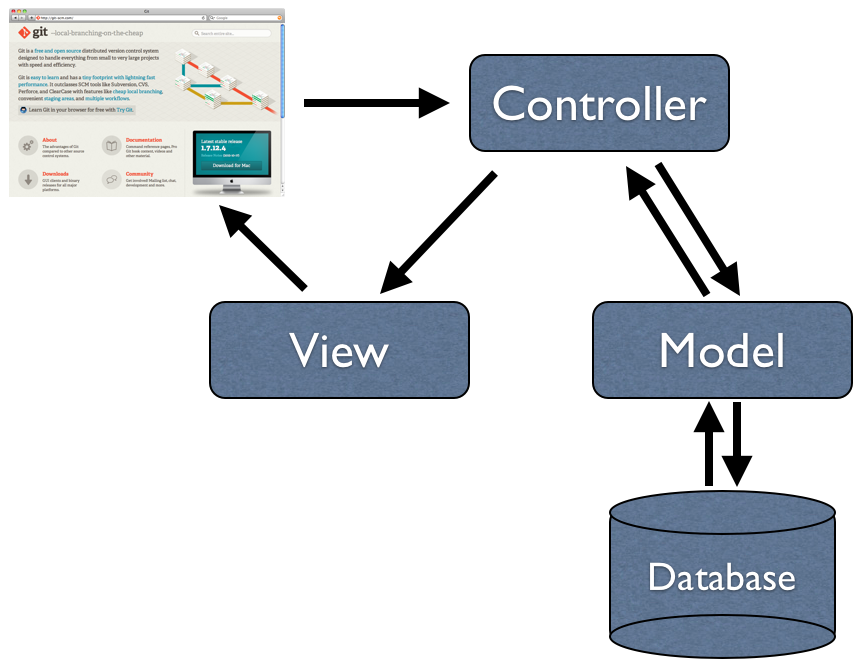
\includegraphics[width=0.9 \textwidth]{figuras/mvc}
    \caption{Esquema MVC}
    \label{figura_23}
\end{figure}

Os modelos são as classes que realizam a persistência, a recuperação e o tratamentos dos dados utilizados pelo sistema, englobando a maior parte da lógica de negócio. No \textit{Rails}, cada modelo está ligado a uma tabela no banco de dados.

As visões são as interfaces de usuário, e devem conter pouca ou nenhuma lógica essencial da aplicação. No \textit{Rails} as views são páginas HTML com código \textit{ruby} incorporado. Na renderização da visão esse código é executado, resultando numa página HTML pura, que será enviada para o navegador do usuário.

Os controladores são responsáveis pela roteamento das requisições da aplicação e por mudanças na interface que não dependam da lógica de negócio, como as interações simples em AJAX. Eles tratam os dados vindos das requisições, se comunicam com os modelos, repassando ou requisitando dados, e finalmente os envia para as visões.
